\documentclass[12pt,letterpaper,DIV=11]{scrartcl}
\usepackage[T1]{fontenc}
\usepackage{amsmath}
\usepackage{amssymb}
\usepackage{amsthm}
\usepackage{booktabs}
\usepackage{hyperref}
\usepackage{mathtools}
\usepackage{microtype}
\usepackage{minted}
\usepackage{csquotes}
\usepackage{multirow}
\usepackage{siunitx}
\usepackage{tikz}
\usepackage{xparse}

\usetikzlibrary{matrix}

\theoremstyle{plain}
\newtheorem{theorem}{Theorem}[section]
%\newtheorem{lemma}[theorem]{Lemma}
\newtheorem{corollary}{Corollary}

\theoremstyle{definition}
%\newtheorem{definition}{Definition}[section]
\newtheorem{example}{Example}[section]

\theoremstyle{remark}
%\newtheorem*{fact}{Fact}
\newtheorem{claim}{Claim}
\newtheorem*{comment}{Comment}

\NewDocumentCommand{\abs}{m}{\left\lvert#1\right\rvert}
\NewDocumentCommand{\norm}{m}{\left\lVert#1\right\rVert}

\DeclareDocumentCommand{\tran}{}{^{\mkern-1.5mu\mathsf{T}}}

\begin{document}
\noindent{}Textbooks:
\begin{itemize}
  \item John Loustau, Elements of Numerical Analysis with \emph{Mathematica}
  \item Eugene Isaacson, Analysis of Numerical Methods
  \item Lloyd Trefethen, Numerical Linear Algebra
\end{itemize}

\begin{displayquote}
  \emph{Numerical analysis is the study of algorithms for the problems of continuous mathematics.}
  \hfill --- Lloyd Trefethen and David Bau
\end{displayquote}
Numerical methods is a branch of mathematics concerned with approximations.
It was founded by John von Neumann and his colleagues in the Manhattan Project during World War II to simulate physical processes governed by differential equations too complex for analytic solutions.

\section{Iterative Solutions of Non-Linear Equations}
We start our survey of numerical methods with a simple introduction to root finding.
This dates back to 1600--1800 BCE (see example Babylonian tablet).

Let $V$ and $W$ be vector spaces.
Our task is to determine roots of the equation $f(x) = 0$, where $f : V \to W$.
What values of $x$ will satisfy this mapping?
Note that:
\begin{itemize}
  \item we are working with non-linear equations; that is, there is no restriction for $f$ to be linear,
  \item we require $\dim(V) = \dim(W) = k$ (when $k = 1$, we have a scalar function of a single variable) as the output becomes the input when we iterate.
\end{itemize}
Suppose we want to find the root of $f(x) = \cos(x)$.
We can reframe the problem to instead find the intersection of $g(x) = x - \cos(x)$ and $y = x$.
This intersection is selected such that the output of $f$ is equal to the input, and thus is called a \textbf{fixed point}.

We will be looking for fixed points of $g$, not roots of $f$.
For now, we can think that $g \equiv x - f(x)$.
If $f(\alpha) = 0$, then $g(\alpha) = \alpha$.

An iterative method gives a series of approximations given an initial approximation called $x_0$.
These iterative methods will be written as
\begin{displaymath}
  x_{i + 1} = g(x_i) \begin{cases}
    \begin{aligned}
      x_1 &= g(x_0) \\
      x_2 &= g(x_1) \\
          &\vdotswithin{=} \\
    \end{aligned}
  \end{cases}
\end{displaymath}

\begin{example}
  Suppose $g(x) = \frac{1}{2} \left( \frac{2}{x} + x \right)$.
  Let $x_0 = 1$.
  Then \begin{displaymath}
    \begin{aligned}
      x_1 &= g(x_0)  \\
          &= \frac{1}{2} \left( \frac{2}{1} + 1 \right) \\
          &= 1.5
    \end{aligned}
    \qquad\qquad
    \begin{aligned}
      x_2 &= g(x_1) \\
          &= \frac{1}{2} \left( \frac{4}{3} + \frac{3}{2} \right) \\
          &= 1.41\overline{6},
    \end{aligned}
  \end{displaymath} and so on.
  We see that $\lim\limits_{i \to \infty} x_i = \sqrt{2}$, and sure enough,
  $g(\sqrt{2}) = \frac{1}{2} \left( \frac{2}{\sqrt{2}} + \sqrt{2} \right) = \sqrt{2}$.
\end{example}
Unfortunately, this method only works when:
\begin{theorem}[Banach fixed-point theorem]\label{thm:banachfpt}
  Given $g$ and $x_0$, if \begin{enumerate}
    \item $g$ takes a closed and bounded set into itself,
    \item $g$ is contracting, i.e. $\norm{g(x) - g(y)} \leq M \norm{x - y}$ with $M < 1$ for all $x, y \in S$ (M is called the Lipschitz constant),
  \end{enumerate}
  then we will converge to a fixed point.
\end{theorem}
This scheme is called a Picard iteration or functional iteration method.
It was originally used to approximate solutions of ordinary differential equations.

Choosing a good $x_0$ is an unresolved problem, but we can usually figure out a good estimate from the problem formulation.

\begin{theorem}[Functional iteration for a single equation (scalar valued)]\label{thm:iterscalar}
  Let $g(x)$ satisfy the Lipschitz condition $\abs{g(x) - g(y)} \leq \lambda \abs{x - y}$ for all $x, y \in I$,
  where $I = [x_0 - \rho, x_0 + \rho]$ and $0 \leq \lambda < 1$ ($\lambda$ is the Lipschitz constant).
  Furthermore, let the original estimate $x_0$ be such that $\abs{x_0 - g(x_0)} \leq (1 - \lambda) \rho$.
  Then the following results hold: \begin{enumerate}
    \item $x_i \in I$ for all $i$,
    \item $\lim\limits_{i \to \infty} x_i = \alpha$ (existence of a fixed point),
    \item $\alpha$ is the only fixed point in $I$ (uniqueness).
  \end{enumerate}

  \begin{proof}\leavevmode
    \begin{enumerate}
      \item We prove $x_i \in I$ by induction.
        \begin{enumerate}
          \item Let $x_0 \in I$.
            Since $g(x_0) = x_1$, we have \begin{align*}
              \abs{x_0 - g(x_0)} &= \abs{x_0 - x_1} \\
                                 &\leq (1 - \lambda) \rho && \text{by our second condition} \\
                                 &\leq \rho && \text{as $0 \leq \lambda < 1$, thus $1 - \lambda < 1$.}
            \end{align*}
          \item Suppose $\abs{x_i - x_0} \leq \rho$ for all $i \leq m$; that is, $x_i \in I$.
            By the Lipschitz condition, we have that for all $i \leq m$, \begin{align*}
              \abs{g(x_i) - g(x_{i - 1})} &\leq \lambda \abs{x_i - x_{i - 1}} \\
                                          &\leq \lambda \abs{g(x_{i - 1}) - g(x_{i - 2})} \\
                                          &\leq \lambda^2 \abs{x_{i - 1} - x_{i - 2}} && \text{again by the Lipschitz condition} \\
                                          &\vdotswithin{\leq} \\
                                          &\leq \lambda^m \abs{x_i - x_0} \\
                                          &\leq \lambda^m (1 - \lambda) \rho.
            \end{align*}
            To show $x_{m + 1} \in I$, consider \begin{align*}
              \abs{x_{m + 1} - x_0} &= \abs{(x_{m + 1} - x_m) + (x_m - x_{m - 1}) + \cdots + (x_1 - x_0)} \\
                                    &\leq \abs{x_{m + 1} - x_m} + \abs{x_m - x_{m - 1}} + \cdots + \abs{x_1 - x_0} \\
                                    &\leq \lambda^m (1 - \lambda) \rho + \lambda^m (1 - \lambda) \rho + \cdots + \lambda^m (1 - \lambda) \rho \\
                                    &= (\lambda^m + \lambda^{m - 1} + \cdots + 1) (1 - \lambda) \rho \\
                                    &= \left( \frac{1 - \lambda^{m + 1}}{1 - \lambda} \right) (1 - \lambda) \rho \\
                                    &= \left( 1 - \lambda^{m + 1} \right) \rho \\
                                    &\leq \rho
            \end{align*} as $0 \leq \lambda < 1$, thus $1 - \lambda < 1$.
        \end{enumerate}
        Thus $x_{m + 1} \in I$, completing the proof by induction.

      \item To show the existence of a limit for the sequence $\{ x_i \}$, we first show that the sequence is Cauchy.
        Given $\epsilon > 0$, we find $N(\epsilon)$ such that for $m, m + p > N$, we have $\abs{x_m -  x_{m + p}} < \epsilon$.
        First, examine \begin{align*}
          \abs{x_m - x_{m + p}} &= \abs{(x_m - x_{m + 1}) + (x_{m + 1} - x_{m + 2}) + \cdots + (x_{m + p - 1} - x_{m + p})}.
          \intertext{By the triangle inequality, we have}
          \abs{x_m - x_{m + p}} &\leq \abs{x_m - x_{m + 1}} + \abs{x_{m + 1} - x_{m + 2}} + \cdots + \abs{x_{m + p - 1} - x_{m + p}} \\
                                &\leq (\lambda^m + \lambda^{m + 1} + \cdots + \lambda^{m + p - 1}) (1 - \lambda) \rho \\
                                &= (1 - \lambda^p) \lambda^m \rho \\
                                &\leq \lambda^m \rho.
        \end{align*}
        So if we want $\abs{x_m - x_{m +p}} < \epsilon$, take $N$ such that $\lambda^N \rho < \epsilon$.
        For instance, let $N = \left\lceil \frac{\log \frac{\epsilon}{p}}{\log \lambda} \right\rceil$.
        Thus we are guaranteed that $\abs{x_m - x_{m + p}} < \epsilon$ for $m, m + p > N$.
        Hence the sequence is Cauchy, and $\lim\limits_{i \to \infty} x_i = \alpha$ since $I$ is a complete metric space.
        %[for homework, show that if $\mathbb{R}$ is complete and $I$ is closed, then $I$ is complete]
        Furthermore, we have that \begin{align*}
          g(\lim_{i \to \infty} x_i) &= \lim_{i \to \infty} g(x_i) && \text{as $g$ is continuous} \\
                                     &= g(\alpha) \\
                                     &= \alpha,
        \end{align*} showing the existence of a fixed point.

        \begin{comment}
          How does $x_i$ approach our fixed point $\alpha$?
          Look at how far our initial guess is from $\alpha$, and the number of iterations we make: \begin{align*}
            \abs{x_m - \alpha} &= \abs{g(x_{m - 1}) - g(\alpha)} \\
                               &\leq \lambda \abs{x_{m - 1} - \alpha} && \text{by the Lipschitz condition} \\
                               &= \lambda \abs{g(x_{m - 2}) - g(\alpha)} \\
                               &\leq \lambda^2 \abs{x_{m - 2} - \alpha} \\
                               &\vdotswithin{\leq} && \text{using the Lipschitz inequality}\\
                               &\leq \lambda^m \abs{x_0 - \alpha} \\
                               &\leq \lambda^m  \rho,
          \end{align*} so each iterate is contained within a smaller and smaller set surrounding $\alpha$.
        \end{comment}

      \item To show uniqueness, suppose $\alpha$ and $\beta$ are both fixed points in $I$.
        Then we have that \begin{align*}
          \abs{\alpha - \beta} &= \abs{g(\alpha) - g(\beta)} \\
                               &\leq \lambda \abs{\alpha - \beta}
        \end{align*} by the Lipschitz condition.
        But since $\lambda < 1$, it must be the case that $\abs{\alpha - \beta} = 0$.
        \qedhere
    \end{enumerate}
  \end{proof}
\end{theorem}


What does this mean for differentiable functions?
Differentiable functions are closely related to Lipschitz, but they are not necessarily Lipschitz.
For example, there is no Lipschitz condition number that will satisfy the inequality for $x^2$, where $x \in \mathbb{R}$.
\begin{corollary}\label{cor:iterscalar}
  If $\abs{g'(x)} \leq \lambda < 1$ for $\abs{x - x_0} \leq \rho$, and $\abs{x_0 - g(x_0)} \leq (1 - \lambda) \rho$, then results (1), (2), and (3) of Theorem~\ref{thm:iterscalar} hold.
  \begin{proof}
    The Mean Value Theorem gives us a way to go between secant lines (our Lipschitz condition) and tangent lines (our differentiable function).
    It states that if $f$ is differentiable on the interval $[a, b]$, then there exists $\xi$ such that $a < \xi < b$ and $f'(\xi) = \frac{f(b) - f(a)}{b - a}$.

    Let $x, y \in I$, and assume $x < y$ without loss of generality.
    By the Mean Value Theorem, we have \begin{align*}
      g(x) - g(y) &= g'(\xi)(x - y) \\
      \abs{g(x) - g(y)} &\leq \lambda \abs{x - y} && \text{since $\abs{g'(\xi)} \leq \lambda$}
    \end{align*} for $x < \xi < y$, so our Lipschitz condition number is at most $\lambda < 1$ for all $x, y \in I$.
    All the results of Theorem~\ref{thm:iterscalar} follow.
  \end{proof}
\end{corollary}

\subsection{Visualizing Iterative Methods}
To understand our convergence theorem, consider $\frac{\Delta y}{\Delta x} = \lambda$ and $\frac{\Delta y}{\Delta x} = - \lambda$ on the interval $[x_0 - \rho, x_0 + \rho]$, both passing through the point $(x_0, g(x_0))$ to form a \enquote{bowtie}.
Notice that at $x = x_0 + \rho$, $g(x) = g(x_0) + \lambda \rho$.
Consider $y = x$, and let $\epsilon = \abs{x_0 - g(x_0)}$.
Then at $x = x_0 + \rho$, we have that the distance between $y = x$ and $\frac{\Delta y}{\Delta x} = \lambda$ is $\rho - \epsilon - \lambda \rho$.
[diagram omitted] % TODO?

If $\lambda > 1$, then our bowtie becomes too tall, and thus $y = x$ does not intersect with the top part of the triangle.
If $\lambda < 1$, but $\rho - \epsilon - \lambda \rho < 0 \iff \epsilon > (1 - \lambda) \rho$, then $y = x$ does not intersect with the top part of the triangle as well.
  Thus $\lambda < 1$ and $\abs{x_0 - g(x_0)} < (1 - \lambda) \rho$ guarantees us a fixed point in $I$.
  There is a second mirrored case discussing the bottom part of the triangle omitted for brevity.

  Why do we want this?
  We need $y = x$ to intersect with the bowtie because that is where $g$ lives, from our Lipschitz condition.
  The premise of fixed points is that our function intersects with $y = x$, the same as how our function intersects with $y = 0$ when root-finding.
  Otherwise, we are not guaranteed that a fixed point exists in this interval, as $g$ could \enquote{escape} in between $y = x$ and the top portion of the bowtie.

  \begin{theorem}[Convergence Theorem 2]\label{thm:convergence2}
    If \begin{enumerate}
      \item[$(\star)$] $g(x)$ has a fixed point $\alpha$ in the interval $I = [\alpha - \rho, \alpha + \rho]$ and
      \item[$(\star\star)$] $g$ satisfies $\abs{g(x) - g(\alpha)} \leq \lambda \abs{x - \alpha}$ for all $x \in I$ with $\lambda < 1$,
      \end{enumerate} then for all choice of $x_0 \in I$, \begin{enumerate}
      \item $x_i \in I$ for all $i$,
      \item $\lim\limits_{i \to \infty} x_i = \alpha$,
      \item the fixed point $\alpha$ is unique in $I$.
    \end{enumerate}
    \begin{proof}\leavevmode
      \begin{enumerate}
        \item We prove $x_i \in I$ by induction. \begin{enumerate}
          \item $x_0 \in I$ by our hypothesis.
          \item $x_i \in I$ for $i \leq m - 1$.
            Since $g(\alpha) = \alpha$, we have \begin{align*}
              \abs{\alpha - x_m} &= \abs{g(\alpha) - g(x_{m - 1})} \\
                                 &\leq \lambda \abs{\alpha - x_{m - 1}} && \text{by hypothesis $(\star\star)$} \\
                                 &\leq \lambda \rho \\
                                 &< \rho && \text{as $\lambda < 1$},
            \end{align*} so $x_m \in I$.
            Furthermore, if we look at these as errors, the $m$\textsuperscript{th} error is bounded above by the $(m - 1)$\textsuperscript{th} error (as $\lambda < 1$).
        \end{enumerate}

      \item We have that \begin{align*}
          \abs{\alpha - x_m} &\leq \lambda \abs{\alpha - x_{m - 1}} \\
                             &\vdotswithin{\leq} && \text{applying $(\star\star)$ recursively} \\
                             &\leq \lambda^m \abs{\alpha - x_0},
          \end{align*} so \begin{align*}
          \lim_{i \to \infty} \abs{\alpha - x_i} &\leq \lim_{i \to \infty} \lambda^i \abs{\alpha - x_0} \\
                                                 &= 0 && \text{since $\lambda^i \to 0$ as $i \to \infty$},
        \end{align*} thus it must be the case that $\lim\limits_{i \to \infty} x_i = \alpha$.

      \item Uniqueness follows as in the proof for Theorem~\ref{thm:iterscalar}.
        \qedhere
    \end{enumerate}
  \end{proof}
\end{theorem}
Now we prove a corollary similar to Corollary~\ref{cor:iterscalar} for Theorem~\ref{thm:iterscalar}.
This will highlight the role of $g'$ in the utility of our iterative scheme.
\begin{corollary}\label{cor:upperboundg'}
  If we replace premise $(\star\star)$ with $\abs{g'(x)} \leq \lambda < 1$ for $x \in I$, then results (1), (2), and (3) of Theorem~\ref{thm:convergence2} hold.
  \begin{proof}
    As in the proof of Corollary~\ref{cor:iterscalar}, we will use the Mean Value Theorem.
    By the Mean Value Theorem, there exists $\xi_{i - 1}$ between $\alpha$ and $x_{i - 1}$ such that \begin{align*}
      g'(\xi_{i - 1}) &= \frac{g(\alpha) - g(x_{i - 1})}{m - x_{i - 1}} \\
                      &= \frac{\alpha - x_i}{\alpha - x_{i - 1}} \\
      \abs{g'(\xi_{i - 1})} \abs{\alpha - x_{i - 1}} &= \abs{\alpha - x_i} \\
      \lambda \abs{\alpha - x_{i - 1}} &\geq  && \text{by our hypothesis.}
    \end{align*}
    Thus our Lipschitz condition is satisfied, and Theorem~\ref{thm:convergence2} will follow.
  \end{proof}
\end{corollary}

\begin{table}
  \centering
  \begin{tabular}{l l l}
    \toprule
  & Theorem~\ref{thm:iterscalar} & Theorem~\ref{thm:convergence2} \\
  \midrule
    \multirow{2}{*}{Conditions} & $\abs{g(x) - g(y)} \leq \lambda \abs{x - y}$ & $\abs{g(x) - g(\alpha)} \leq \lambda \abs{x - \alpha}$ \\
                                & $\abs{x_0 - g(x_0)} \leq (1 - \lambda) \rho$ & $x_0 \in I$ \\
                                \midrule
    Result & $\exists! \alpha$ & $\lim\limits_{i \to \infty} \lambda_i = \alpha$ for all $x_0 \in I$ \\
    \bottomrule
  \end{tabular}
  \caption{Differences between Theorem~\ref{thm:iterscalar} and Theorem~\ref{thm:convergence2}.}
\end{table}

$g'$ is important because it stands in as our Lipschitz condition number.
When the condition number is smaller, we assume that our iterates approach our fixed point quicker.

If $x_i$ converges to $\alpha$, then $\xi_i$ converges to $\alpha$ as well as it is is between $x_i$ and $\alpha$.
From this convergence and our previous Mean Value Theorem iterated, \begin{align*}
  \abs{\alpha - x_{k + m}} &= \abs{g'(\xi_{k + m - 1})} \abs{\alpha - x_{k + m - 1}} \\
                           &\vdotswithin{=} \\
                           &= \abs{g'(\xi_{k + m - 1})} \dots \abs{g'(\xi_k)} \abs{\alpha - x_k} \\
                           &\approx \abs{g'(\alpha)}^m \abs{\alpha - x_k}
\end{align*} for large enough $x_i$ so that $\xi_k$ is close to $\alpha$.
Thus our iterates get closer by approximately a factor of $g'(\alpha)$ each iteration.

We call $\hat{\lambda} \equiv \abs{g'(\alpha)}$ the (asymptotic) convergence factor.
When $g'(\alpha) \neq 0$, $g$ is a first order method.

\subsection{Error Propagation}
When computing $g(x)$, we will be limited by machine precision.
Given a values $x$, we represent our approximation of $g(x)$ by $G(x) = g(x) + \delta(x)$, where $\delta(x)$ is the error committed when we evaluate.

\begin{example}
  Let $g(x) = \frac{x}{3}$.
  Then $g(1) = \frac{1}{3}$, but if $G(1) = 0.33$, then $\delta(1) = 0.00\bar{3}$.
\end{example}
In practice, we can obtain a bound $\delta$ on $\delta(x)$.
For our iteration schemes, we write $X_{i + 1} = g(X_i) + \delta_i$, where $i = 0, 1, 2, \dots$,
where $X_i$ are the calculated iterates and $\delta_i$ are the errors added each iteration.
Because we cannot store infinite digits (that is, $\delta_i$ is always present), we cannot expect $X_i$ to converge all the time.

We still expect $X_i$ to approximate a fixed point.
The accuracy of the approximation is determined by $\delta$, the maximum value of the error term.

\begin{example}
  Let $g(x) = \alpha + \lambda (x - \alpha)$.
  We can easily verify that our fixed point is $g(\alpha) = \alpha$.
  Observe that $y = g(x) - \delta$ intersects $y = x$ at $x = \alpha - \frac{\delta}{1 - \lambda}$ and $y = g(x) + \delta$ intersects $y = x$ at $x = \alpha + \frac{\delta}{1 - \lambda}$.
  Thus our uncertainty in $\alpha$ lies in the range $\pm \frac{\delta}{1 - \lambda}$.

  If $\lambda$ is close to 1, then the range of uncertainty becomes large!
  Our estimates of $g(x)$ might leave $I$.
  We say that the problem isn't \enquote{properly posed} if $\lambda$ is close to 1.
\end{example}

\begin{theorem}[Error propagation theorem]
  Let $g$ satisfy the conditions of Theorem~\ref{thm:convergence2}
  Let $X_0$ be any point \begin{enumerate}
    \item[$(\star)$] in the interval $I = [\alpha - \rho_0, \alpha + \rho_0]$,
    \item[$(\star\star)$] where $\rho_0$ is given by $0 < \rho_0 \leq \rho - \frac{\delta}{1 - \lambda}$ (taking care of the \enquote{properly posed} problem).
  \end{enumerate}
  Then the iterates $X_i$ with errors bounded by $\delta$ lie in the interval $\abs{\alpha - X_i} < \rho$ and $\abs{\alpha - X_i} \leq \frac{\delta}{1 - \lambda} + \lambda^i \left( \rho_0 - \frac{\delta}{1 - \lambda} \right)$.

  \begin{proof}
    We prove $X_i \in I$ by induction.
    \begin{enumerate}
      \item First show $X_0 \in I$.
        By rearranging premise $(\star\star)$, we get \begin{align*}
          \abs{\alpha - X_0} &\leq \rho_0 && \text{by condition $(\star)$} \\
                             &\leq \rho_0 + \frac{\delta}{1 - \lambda} && \text{as $\frac{\delta}{1 - \lambda}$ is positive} \\
                             &\leq \rho - \frac{\delta}{1 - \lambda} + \frac{\delta}{1 - \lambda} && \text{by condition $(\star\star)$} \\
                             &= \rho.
        \end{align*}

      \item Now assume $X_i \in I$ for $i \leq m - 1$.
        \begin{align*}
          \abs{\alpha - X_m} &= \abs{g(\alpha) - \left[ g(X_{m - 1}) + \delta_{m - 1} \right]} \\
                             &\leq \abs{g(\alpha) - g(X_{m - 1})} + \abs{-\delta_{m - 1}} && \text{by the triangle inequality} \\
                             &\leq \lambda \abs{\alpha - X_{m - 1}} + \delta \\
                             &\leq \lambda^2 \abs{\alpha - X_{m - 2}} + \lambda \delta  + \delta && \text{by our Lipschitz condition} \\
                             &\vdotswithin{\leq} \\
                             &\leq \lambda^m \abs{\alpha - X_0} + \lambda^{m - 1} \delta + \cdots + \lambda \delta + \delta \\
                             &= \lambda^m \rho_0 + \left( \frac{1 - \lambda^m}{1 - \lambda} \right) \delta \\
                             &= \frac{\delta}{1 - \lambda} - \lambda^m \left( \rho_0 - \frac{\delta}{1 - \lambda} \right) && \text{giving us the second result}.
        \end{align*}
        This separates the computational error from the $m$-dependent terms.
    \end{enumerate}
    We still must prove the first result.
    Continuing from before distributing \begin{align*}
      \abs{\alpha - X_i} &\leq \lambda^i \rho_0 + \left( \frac{1 - \lambda^i}{1 - \lambda} \right) \delta \\
                         &= \lambda^i \rho_0 + \frac{\delta}{1 - \lambda} - \lambda^i \frac{\delta}{1 - \lambda} \\
                         &\leq \rho_0 + \frac{\delta}{1 - \lambda} \\
                         &\leq \rho && \text{by premise $(\star\star)$.}
    \end{align*}
    Therefore, $X_i \in I$, and our process is well-defined.
  \end{proof}
\end{theorem}

\subsection{Understanding convergence factor}
How does the convergence factor relate to the number of iterations we need?
From Theorem~\ref{thm:convergence2} we have $\abs{\alpha - X_{m + k}} \approx \hat{\lambda}^k \abs{\alpha - X_m}$.
To increase accuracy by $10^{-m}$, we need $\frac{\abs{\alpha - X_{m + k}}}{\abs{\alpha - X_m}} = 10^{-m} \approx \hat{\lambda}^k$, so $k = \frac{m}{\log \frac{1}{\hat{\lambda}}}$.
Taking into account the resolution from machine precision, we only need to iterate up to \begin{displaymath}
  \min\left( \frac{m}{\log \frac{1}{\hat{\lambda}}}, \underbrace{\frac{\log \frac{\delta}{(1 - \hat{\lambda}) \rho_0}}{\log \hat{\lambda}}}_\text{resolution bound} \right)
\end{displaymath} times.
However, we can take fewer iterates by breaking this condition from our first order methods: $\hat{\lambda} = \abs{g'(\alpha)} \neq 0$.

\section{Second and higher order iteration methods}
To get an intuition of why this helps, suppose $g'(\alpha) = 0$.
If the slope at our fixed point is zero, we expect the slope around the fixed point to be close to zero, i.e.\ $0 < \abs{g'(x)} \ll 1$ (much less than 1) around $\alpha$.

Furthermore, we will assume that $g'(\alpha) = 0$ and $g''(x)$ exists and is bounded in $I \equiv [\alpha - \rho, \alpha + \rho]$.
Then for all $x \in I$, we can use Taylor expansion to get \begin{align*}
  g(x) &= g(\alpha) + g'(\alpha)(x - \alpha) + g''(\xi) \frac{{(x - \alpha)}^2}{2} \\
       &= g(\alpha) + g''(\xi) \frac{{(x - \alpha)}^2}{2} && \text{by our first assumption} \\
       &= \alpha + g''(\xi) \frac{{(x - \alpha)}^2}{2}
\end{align*} where $\xi$ is between $x$ and $\alpha$ by Taylor's theorem due to our second assumption.

From this result, for any $i > 0$, \begin{align*}
  \underbrace{\abs{x_i - \alpha}}_\text{$i$\textsuperscript{th} error} &= \abs{g(x_{i - 1}) - g(\alpha)} \\
                                                                       &= \abs{\alpha - g''(\xi_{i - 1}) \frac{{(x_{i - 1} - \alpha)}^2}{2} - \alpha} \\
                                                                       &= \frac{1}{2} \underbrace{\left\vert g''(\xi_{i - 1}) \right\vert}_\text{bounded} {\underbrace{\left\vert x_{i - 1} - \alpha \right\vert}_\text{previous error}}^2
\end{align*} which is a significant improvement.

Assuming that $g''(\alpha) \neq 0$, we call this a second order method.

\subsection{Convergence Factor and Error Propagation}
Let the bound on $g''$ be denoted as $\abs{g''(x)} \leq 2M$ for all $x \in I$.
Then \begin{align*}
  \underbrace{\abs{x_i - \alpha}}_\text{$i$\textsuperscript{th} error} &\leq \frac{1}{2} (2M) \abs{x_{i - 1} - \alpha}^2 \\
                                                                       &= M \abs{x_{i - 1} - \alpha}^2 \\
                                                                       &\leq M \cdot M^2 \abs{x_{i - 2} - \alpha}^4 \\
                                                                       &\leq M \cdot M^2 \cdot M^4 \abs{x_{i - 3} - \alpha}^8 \\
                                                                       &\vdotswithin{\leq} && \text{using Taylor expansion} \\
                                                                       &\leq M^{2^i - 1} \abs{x_0 - \alpha}^{2^i} \\
                                                                       &\leq {(M \abs{x_0 - \alpha})}^{2^i - 1} \underbrace{\abs{x_0 - \alpha}}_\text{initial error},
\end{align*}
so we converge if $M \abs{x_0 - \alpha} = \hat{\lambda} < 1$.

Suppose we wanted to reduce error by at least $10^{-m}$.
Then $\abs{X_{i + k} - \alpha} \leq 10^{-m} \abs{X_i - \alpha}$, and thus $k \approx \frac{1}{\log 2} \log \frac{m}{\log \left( \hat{\lambda} \frac{1}{\rho} \right)}$.

\subsection{Comparison to the first order scheme}
To get equal reduction of error between our first order scheme conversion factor $\hat{\lambda}_1$ and our second order scheme conversion factor $\hat{\lambda}_2$, $\hat{\lambda}_1^{k_1} = \hat{\lambda}_2^{2^{k_2}}$.
In Corollary~\ref{cor:upperboundg'} we thought of $\hat{\lambda}_1$ as $g'$, and now we think of $\hat{\lambda}_2$ as $g'' \rho$.
Assuming $\hat{\lambda}_1 = \hat{\lambda}_2$, it is easy to see that $k_1 = 2^{k_2}$, which means we need to do $2^{k_2}$ iterations to get the same reduction of error using the first order scheme.
For example, if we need 5 more iterations to get the necessary increase in precision using the second order scheme, this translates to needing 32 more iterations with the first order scheme to see the same improvement.
This basically means that the second order scheme is exponentially better than the first.

\begin{example}
  Find the root of $f(x) = x^2 - 2$.
  \begin{displaymath}
    \begin{array}{c c}
      \toprule
      \text{First order scheme} & \text{Second order scheme} \\
      \midrule
      \begin{aligned}
        g'_1(x) &= x - \frac{1}{2} (x^2 - 2) \\
        g'_1(x) &= 1 - x \\
        g'_1(\sqrt{2}) &= 1 - \sqrt{2}
      \end{aligned} &
      \begin{aligned}
        g_2(x) &= \frac{x}{2} + \frac{1}{x} \\
        g'_2(x) &= \frac{1}{2} - \frac{1}{x^2} \\
        g'_2(\sqrt{2}) &= \frac{1}{2} - \frac{1}{2} = 0
      \end{aligned} \\
      \bottomrule
    \end{array}
  \end{displaymath}
  Let $x_0 = 1$.
  Then we get the following values for $g_1$ and $g_2$, assuming rounding to 5 digits:
  \begin{table}[h]
    \centering
    \begin{tabular}{l S S}
      \toprule
      Iteration & {$g_1$} & {$g_2$} \\
      \midrule
      $x_0$ & 1. & 1. \\
      $x_1$ & 1.5 & 1.5 \\
      $x_2$ & 1.375 & 1.4167 \\
      $x_3$ & 1.42969 & 1.41422 \\
      $x_4$ & 1.40768 & 1.41421 \\
      $x_5$ & 1.4169 & 1.41421 \\
      $x_6$ & 1.4131 & 1.41421 \\
      $x_7$ & 1.41467 & 1.41421 \\
      $x_8$ & 1.41402 & 1.41421 \\
      $x_9$ & 1.41429 & 1.41421 \\
      $x_{10}$ & 1.41418 & 1.41421 \\
      \bottomrule
    \end{tabular}
  \end{table}

  Notice that $g_2$ is already accurate to 2 decimal places by the second iteration, and accurate to 5 decimal places by the fourth iteration, while $g_1$ requires many more iterations to reach that accuracy.
  It turns out that for every iteration of a second order scheme, the number of correct digits doubles, assuming $M < 1$ (when $M > 1$ it is asymptotically true).

  \begin{proof}
    Assume that $\abs{x_m - \alpha} \leq 10^{-k_m}$ for all $m \geq m_0$; i.e.\ past this point, our iterates are correct to $k_m$ decimals.
    Then we have that \begin{align*}
      \abs{x_m - \alpha} &\leq M {\left\vert x_{m - 1} - \alpha \right\vert}^2 \\
      10^{-k_m} &\leq M \cdot 10^{-2k_{m - 1}}
    \end{align*} or $k_m \geq {2 k_{m - 1}}^{-\log M}$,
    so for $M < 1$ we have $-\log M > 0$.
    Thus the number of correct decimals \emph{more than doubles} each iteration (which is only asymptotically true when $M > 1$).
  \end{proof}

  In practice, we want to check the convergence criterion; that is, $g'(x) < 1$ in $I \equiv [\sqrt{2} - \rho, \sqrt{2} + \rho]$.
\end{example}

\subsection{Higher order schemes}
Imagine what would happen in an even better case scenario.
Following the same pattern, assume $g'(\alpha) = g''(\alpha) = \cdots = g^{(n - 1)}(\alpha) = 0$ and $g^{(n)}(\alpha) \neq 0$, with $\abs{g^{(n)}(x)} \leq n!\, M$
in $\abs{x - \alpha} \leq \rho$.
Now consider $g(x) = \alpha + g'(\alpha)(x - \alpha) + \cdots + g^{(n)}(\xi) \frac{{(x - \alpha)}^n}{n!}$, where $\xi$ is between $x$ and $\alpha$ and all intermediate terms are 0 by our first assumption.
Then as from before, we can express our $i$\textsuperscript{th} error as \begin{align*}
  \abs{x_{i + 1} - \alpha} &= \frac{\abs{g^{(n)}(\xi_i)}}{n!} \abs{x_i - \alpha}^n \\
                           &\leq M \abs{x_i - \alpha}^n
\end{align*} by our second assumption, giving us our convergence factor.
This is called an $n$\textsuperscript{th} order procedure.
It multiplies the number of correct decimals by $n$ each iteration (at least asymptotically).

\subsubsection{Error propagation}
Since $g'(\alpha) = 0$, then the upper bound $\lambda$ is close to 0, so the fudge factor $\pm \frac{\delta}{1 - \delta}$ becomes $\pm \delta$.
Thus error propagation isn't really a concern with higher order procedures.

\section{Explicit iteration procedures}
Going back to the original task of finding roots of any scalar equation $f(x) = 0$ in some interval $a \leq x \leq b$,
let $\phi(x)$ be any function such that $0 < \abs{\phi(x)} < \infty$.
Now our placeholder function $g \equiv x - f(x)$ will be $g(x) \equiv x - \phi(x) f(x)$.
Is this suitable for root finding (i.e.\ does a fixed point in $g$ yield a root in $f$)?
Assuming $g(\alpha) = \alpha$, we get $\alpha = \alpha - \phi(\alpha) f(\alpha)$; that is, $\phi(\alpha) f(\alpha) = 0$.
Since $0 < \abs{\phi(x)}$, the only factor that can approach 0 is $f(\alpha)$, so $\alpha$ is a root of $f$.
There are many different choice of $\phi(x)$ that will lead to different iterative procedures.

An alternative method of going from fixed point to root is composition.
Let $g(x) \equiv x - F(f(x))$, where $F$ is a function such that $F(y) = 0$ if and only if $y = 0$.
Composition methods often describe higher order schemes.

\subsection{Chord Method}
The simplest choice for $\phi(x)$ is to let $\phi(x) \equiv m \neq 0$, where $m \in \mathbb{R}$.
If $f$ is differentiable, by Corollary~\ref{cor:iterscalar}, we get convergence when $\abs{g'(x)} < 1$.
Looking at $g'$, we see that \begin{align*}
  g(x) &= x - m f(x) \\
  g'(x) &= 1 - m f'(x),
\end{align*}
so for convergence, \begin{equation}
  \abs{g'(x)} = \abs{1 - m f'(x)} < 1
\end{equation} or
\begin{equation}\label{eqn:chordconvergence2}
  0 < m f'(x) < 2.
\end{equation}
From these inequalities, we see that $m$ must have the same parity as $f'$, and if $f'(x) = 0$, then the convergence condition cannot be satisfied.
This means that it does not work for higher order schemes, and we don't want $f$ to be constant in our interval when using this method.

\subsubsection{Visualizing the chord method}
By $x_{i + 1} = g(x_i)$, we have $x_{i + 1} = x_i - m f(x_i)$.
Given the point $p_i = (x_i, f(x_i))$, we use the point-slope formula to find the line starting at $p_i$ with slope $s$ is $y - f(x_i) = s (x - x_i)$.
Suppose the line has an $x$-intercept of $x_{i + 1}$.
Then it also goes through $(x_{i + 1}, 0)$ and we see that \begin{align*}
  - f(x_i) &= s (x_{i + 1} - x_i) \\
           &= s (-m f(x_i)) && \text{rearranging $x_{i + 1} = x_i - m f(x_i)$ from above} \\
  1 &= sm;
\end{align*} i.e.\ the slope of the line is $\frac{1}{m}$.
Thus the next iteration is the $x$-intercept of the line that passes through the previous iteration's point with a slope of $\frac{1}{m}$.
Eventually this will yield a root.

Note that from Equation~\ref{eqn:chordconvergence2}, we have $\frac{1}{2} f'(x) < \frac{1}{m} < \infty$, which means our slope is greater than half of the tangent line and is not vertical.

\subsubsection{Implementation in Mathematica}
\begin{minted}[mathescape]{mathematica}
f[x_] := x^2 - 2; (* the method we want to find the root of *)
g[x_] := x - 0.5 * f[x]; (* if it doesn't converge, make $m$ (0.5) smaller *)

a = 10; (* Initial guess $x_0$ *)
thresh = 10^(-3); (* residual kick out threshold *)
maxiter = 10; (* maximum number of iterations *)
For[iter = 0, iter < maxiter && Abs[f[a]] > thresh, a = g[a]; Print[a]; iter++]
\end{minted}

\subsection{Newton's Method}
Suppose we are able to adapt the slope of our chord each iteration, so that $g'(x_i) = 1 - \phi(x_i) f'(x_i) = 0$.
Then we have a second order method.
The only choice we have for $\phi$ is $\phi(x) = \frac{1}{f'(x)}$, so $g(x) = x - \frac{\phi(x)}{f'(x)}$.
Observe that with this, we must have $f'(x) \neq 0$ for all $x \in I$.

\subsubsection{Visualization}
Our visualization follows right from the Chord Method, except the chord now has a slope of $\frac{1}{f'(x)}$, tangent to each point.
The lines adjust to look for the root rather than being always parallel.


\subsection{Method of False Position}
So far we've only seen root-solving applications, but this analysis is usually used for solving differential equations.
Sometimes it's not straightforward how to evaluate $f'$, which happens with ordinary differential equations when $f$ is not explicitly given.
However, we can approximate derivatives using divided differences.

Using a secant approximation of $m = \frac{1}{f'(x_i)}$ instead of tangent lines,
we get the procedure \begin{equation}\label{eqn:falseposition}
  x_{i + 1} = x_i - f(x_i) \frac{x_i - x_{i - 1}}{f(x_i) - f(x_{i - 1})}
\end{equation} for $i \in \mathbb{N}$.
Note that we need two successive iterations to calculate $x_{i + 1}$, unlike in Newton's Method, where we only need one.
This means we cannot write our procedure as $x_{i + 1} = g(x_i)$ anymore and therefore will need to express it as some $h(x_i, x_{i - 1})$.
To examine this, let $\alpha$ be a root of $f(x) = 0$.
Then from Equation~\ref{eqn:falseposition} we have \begin{equation}
  \begin{split}\label{eqn:divdiff}
    \alpha - x_{i + 1} &= \left( \alpha - x_i \right) + f(x_i) \frac{x_i - x_{i - 1}}{f(x_i) - f(x_{i - 1})} \\
                       &= \left( \alpha - x_i \right) \frac{f[x_{i - 1}, x_i] - f[x_i, \alpha]}{f[x_{i - 1, x_i}]} \\
                       &= (\alpha - x_i) (\alpha - x_{i - 1}) \left( - \frac{f[x_{i - 1}, x_i, \alpha]}{f[x_{i - 1}, x_i]} \right)
  \end{split}
\end{equation}
where $f[a, b] \equiv \frac{f(b) - f(a)}{b - a}$ is the first divided difference and $f[x_{i - 1}, x_i, \alpha] \equiv \frac{f[x_{i - 1}, x_i] - f[x_i, \alpha]}{x_{i - 1} - \alpha}$ is the second divided difference.

If $f$ has a continuous second derivative in an interval including the points $x_i$, $x_{i - 1}$, and $\alpha$, then by Taylor's Theorem there exists $\xi_i$ and $\eta_i$  such that $f[x_{i - 1}, x_i] = f'(\xi_i)$ and $f[x_{i - 1}, x_i, \alpha] = \frac{1}{2} f''(\eta_i)$.
So by Equation~\ref{eqn:divdiff} we have \begin{displaymath}
  \alpha - x_{i + 1} = \frac{f''(\eta_i)}{2 f'(\xi_i)} (\alpha - x_i) (\alpha - x_{i - 1})
\end{displaymath} for $i \in \mathbb{N}$,
assuming $x_i \in I \equiv [\alpha - \rho, \alpha + \rho]$ for all $i$ and
$\abs{\frac{f''(\eta)}{2 f'(\xi)}} \leq M < \frac{1}{\rho}$ for $\eta, \xi \in I$.

Let $e_i \equiv M \abs{\alpha - x_i}$, then we have \begin{align*}
  \abs{\alpha - x_{i + 1}} &= \abs{\frac{f''(\eta_i)}{2 f'(\xi_i)}} \abs{\alpha - x_i} \abs{\alpha - x_{i - 1}} \\
  \frac{e_{i + 1}}{M} &\leq M \cdot \frac{e_i}{M} \cdot \frac{e_{i - 1}}{M} \\
  e_{i + 1} &\leq e_i e_{i - 1}.
\end{align*}
This says that the subsequent error is bounded by the product of the two previous errors.

Define $\delta \equiv \max(e_0, e_1)$, then we can continue and get the inequalities \begin{align*}
  e_0 &\leq \delta \\
  e_1 &\leq \delta \\
  e_2 &\leq \delta^2 \\
  e_3 &\leq \delta^3 \\
  e_4 &\leq \delta^5 \\
      &\vdotswithin{\leq} \\
  e_i &\leq \delta^{m_i}
\end{align*} where $m_0 = m_1 = 1$ and $m_{i + 1} = m_i + m_{i - 1}$; i.e. $m_i$ is the $i$\textsuperscript{th} element of the Fibonacci sequence.
We call this a golden ratio order procedure as our errors go to zero at an order of roughly 1.618.

\section{Systems of Linear Equations}
Now we look at systems of linear equations: many simple equations that have to be satisfied concurrently.
It turns out that many mathematical problems boil down to just solving a system of linear equations.

\begin{example}
  Michael buys two bags of chips and three boxes of pretzels for \$7.
  He then buys another bag of chips and two more boxes of pretzels for \$4.
  Find the cost of each bag of chips and each box of pretzels.

  Let $c$ be the price of one bag of chips and $p$ the price of one box of pretzels.
  Recall that scalar multiplication and addition are linear operations, and two equations have to be satisfied at the same time, hence this is a system of two linear equations: \begin{align*}
    2c + 3p &= 7 \\
    c + 2p &= 4,
  \end{align*} which can be solved by reframing in terms of matrices and vectors such that $A \vec{x} = \vec{b}$, where $A$ is the coefficient matrix, $\vec{x}$ is a vector of unknowns (or solutions), and $\vec{b}$ is a vector of constants:
  \begin{displaymath}
    \begin{bmatrix}
      2 & 3 \\
      1 & 2
    \end{bmatrix}
    \begin{bmatrix}
      c \\
      p
    \end{bmatrix} =
    \begin{bmatrix}
      7 \\
      4
    \end{bmatrix}.
  \end{displaymath}
  This equation could be solved by hand using Gaussian Elimination.
\end{example}

\subsection{LU Factorization}
Gaussian Elimination takes nonsingular (invertible) linear systems and gives an upper triangular one by applying simple linear transformations.

An upper triangular matrix $U$ has $u_{ij} = 0$ when $i > j$ (zeros beneath the main diagonal), while a lower triangular matrix $L$ has $l_{ij} = 0$ when $i < j$ (zeros above the main diagonal).
Solving the system of linear equations above becomes quite simple once $A$ has been factored into its $L$ and $U$ components.


Let $A \in \mathbb{C}^{m \times m}$ be a square matrix.
To go from $A$ to $U$ we need to introduce zeros below the diagonal.
This \enquote{elimination} is done column by column, from left to right, by multiplying lower triangular matrices (linear transformations) on the left of $A$.
The process essentially applies linear transformations to the system of linear equations in order to make a different system that is easier to solve: \begin{align*}
  L_{m - 1} \cdots L_2 L_1 A &= U && \text{where $L_i$ has zeros in column $i$} \\
  A &= L_1^{-1} L_2^{-1} \cdots L_{m - 1}^{-1} U \\
  A &= LU && \text{where $L = L_1^{-1} \cdots L_{m - 1}^{-1}$}.
\end{align*}
Having the actual factorization of $A$ isn't necessary, but can be helpful in some other aspects.
We will see $L$ is lower triangular due to the nature of these linear transformations.

\begin{figure}[h]
  \centering
  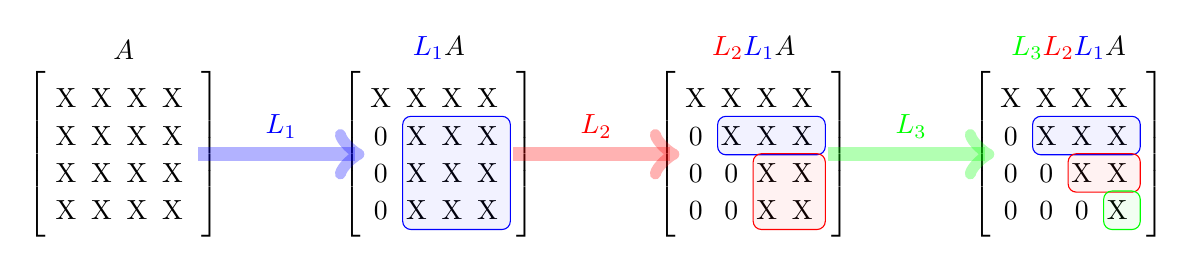
\begin{tikzpicture}[
    auto,
    Matrix/.style={matrix of nodes,align=center,left delimiter={[},right delimiter={]},inner xsep=1pt},
    Highlight/.style={fill,rounded corners=3pt,fill opacity=0.05},
    Line/.style={->,line width=5pt,draw opacity=0.3},
    ]

    \matrix[Matrix,label=$A$] at (0,0) (A) {
      X & X & X & X \\
      X & X & X & X \\
      X & X & X & X \\
      X & X & X & X \\
    };
    \matrix[Matrix,label=$\textcolor{blue}{L_1} A$] at (4,0) (LA) {
      X & X & X & X \\
      0 & X & X & X \\
      0 & X & X & X \\
      0 & X & X & X \\
    };
    \matrix[Matrix,label=$\textcolor{red}{L_2} \textcolor{blue}{L_1} A$] at (8,0) (LLA) {
      X & X & X & X \\
      0 & X & X & X \\
      0 & 0 & X & X \\
      0 & 0 & X & X \\
    };
    \matrix[Matrix,label=$\textcolor{green}{L_3} \textcolor{red}{L_2} \textcolor{blue}{L_1} A$] at (12,0) (LLLA) {
      X & X & X & X \\
      0 & X & X & X \\
      0 & 0 & X & X \\
      0 & 0 & 0 & X \\
    };

    \draw[Highlight,blue]  (  LA-2-2.north west) rectangle (  LA-4-4.south east);
    \draw[Highlight,blue]  ( LLA-2-2.north west) rectangle ( LLA-2-4.south east);
    \draw[Highlight,red]   ( LLA-3-3.north west) rectangle ( LLA-4-4.south east);
    \draw[Highlight,blue]  (LLLA-2-2.north west) rectangle (LLLA-2-4.south east);
    \draw[Highlight,red]   (LLLA-3-3.north west) rectangle (LLLA-3-4.south east);
    \draw[Highlight,green] (LLLA-4-4.north west) rectangle (LLLA-4-4.south east);

    \draw[Line,blue]    (A) -- (LA) node   [midway,above] {\textcolor{blue}  {$L_1$}};
    \draw[Line,red]    (LA) -- (LLA) node  [midway,above] {\textcolor{red}   {$L_2$}};
    \draw[Line,green] (LLA) -- (LLLA) node [midway,above] {\textcolor{green} {$L_3$}};
  \end{tikzpicture}
  \caption{The linear transformations performed when factoring a $4 \times 4$ matrix $A$ into its upper triangular form.
    Non-zero values are represented by $X$, with highlighted regions showing which values change as linear transformations are applied.
  }
\end{figure}

In general, the $k$\textsuperscript{th} linear transformation introduces zeros below the diagonal in column $k$.
It does this by subtracting multiples of row $k$ from rows under row $k$.
Since columns $1, \dots, k$ already have zeros in the proper location, the transformation does not introduce nonzeros into those elements.

\begin{example}
  Now that we understand shape, let \begin{displaymath}
    A = \begin{bmatrix}
      2 & 1 & 1 & 0 \\
      4 & 3 & 3 & 1 \\
      8 & 7 & 9 & 5 \\
      6 & 7 & 9 & 8
    \end{bmatrix}.
  \end{displaymath}
  The first step is to introduce zeros into the first column: \begin{displaymath}
    L_1 A = \underbrace{\begin{bmatrix*}[r]
        1 & 0 & 0 & 0 \\
        -2 & 1 & 0 & 0 \\
        -4 & 0 & 1 & 0 \\
        -3 & 0 & 0 & 1
    \end{bmatrix*}}_{L_1}
    \underbrace{\begin{bmatrix}
        2 & 1 & 1 & 0 \\
        4 & 3 & 3 & 1 \\
        8 & 7 & 9 & 5 \\
        6 & 7 & 9 & 8
    \end{bmatrix}}_A =
    \begin{bmatrix}
      2 & 1 & 1 & 0 \\
      0 & 1 & 1 & 1 \\
      0 & 3 & 5 & 5 \\
      0 & 4 & 6 & 8
    \end{bmatrix},
  \end{displaymath}
  then do the same with the second column: \begin{displaymath}
    L_2 L_1 A = \underbrace{\begin{bmatrix*}[r]
        1 & 0 & 0 & 0 \\
        0 & 1 & 0 & 0 \\
        0 & -3 & 1 & 0 \\
        0 & -4 & 0 & 1
    \end{bmatrix*}}_{L_2}
    \underbrace{\begin{bmatrix}
        2 & 1 & 1 & 0 \\
        0 & 1 & 1 & 1 \\
        0 & 3 & 5 & 5 \\
        0 & 4 & 6 & 8
    \end{bmatrix}}_{L_1 A} =
    \begin{bmatrix}
      2 & 1 & 1 & 0 \\
      0 & 1 & 1 & 1 \\
      0 & 0 & 2 & 2 \\
      0 & 0 & 2 & 4
    \end{bmatrix},
  \end{displaymath}
  and the third column: \begin{displaymath}
    L_3 L_2 L_1 A =
    \underbrace{\begin{bmatrix*}[r]
        1 & 0 & 0 & 0 \\
        0 & 1 & 0 & 0 \\
        0 & 0 & 1 & 0 \\
        0 & 0 & -1 & 1
    \end{bmatrix*}}_{L_3}
    \underbrace{\begin{bmatrix}
        2 & 1 & 1 & 0 \\
        0 & 1 & 1 & 1 \\
        0 & 0 & 2 & 2 \\
        0 & 0 & 2 & 4
    \end{bmatrix}}_{L_2 L_1 A} =
    \begin{bmatrix}
      2 & 1 & 1 & 0 \\
      0 & 1 & 1 & 1 \\
      0 & 0 & 2 & 2 \\
      0 & 0 & 0 & 2
    \end{bmatrix}.
  \end{displaymath}
\end{example}
It is trivial to compute $L = L_1^{-1} L_2^{-1} L_3^{-1}$, as the inverse of a matrix in this form is simply the non-diagonal elements negated, so: \begin{displaymath}
  L = \begin{bmatrix}
    1 & 0 & 0 & 0 \\
    2 & 1 & 0 & 0 \\
    4 & 3 & 1 & 0 \\
    3 & 4 & 1 & 1
  \end{bmatrix}.
\end{displaymath}

\subsubsection{General Formula}
Suppose $x_k$ denotes the $k$\textsuperscript{th} column of the matrix.
Choose $L_k$ so that there are zeros everywhere below the diagonal element $x_{k k}$.
To do this, subtract $l_{jk}$ multiplied by row $k$ from row $j$, where $l_{jk} = \frac{x_{jk}}{x_{kk}}$ (the element to get rid of divided by the diagonal element) for all $j > k$.
We can verify that \begin{align*}
  L_k \cdot x_{k} &= -l_{k + 1, k} \cdot x_{kk} + i1 \cdot x_{k + 1, k} \\
                  &= - \frac{x_{k + 1, k}}{x_{kk}} \cdot x_{kk} + x_{k + 1,k} && \text{by the definition of $l$ above} \\
                  &= - x_{k + 1, k} + x_{k + 1,k} \\
                  &= 0,
\end{align*} which is what we expected.

\begin{claim}
  Two nice properties allow for a quick lower triangular matrix factorization:
  $L_k$ can be inverted by negating the subdiagonal entries ($l_{jk}^{-1} = -l_{jk}$ for $j > k$), and
  $L$ can be formed by inserting $L_k$ into $I$ below the diagonal (creating a matrix with $l_{jk}$ in the subdiagonal and 1 on main diagonal).

  \begin{proof}
    Define $l_k = \begin{bmatrix}
      0 & \cdots & 0 & l_{k + 1, k} & \cdots & l_{mk}
    \end{bmatrix}\tran$, which is the $k$\textsuperscript{th} transformation without the 1 in the diagonal element.
    This gives us the nice representation $L_k = I - l_k \cdot e_k\tran$, where $e_k$ is the standard basis vector.
    Note that $l_k$ is a $m \times 1$ matrix, and $e_k\tran$ is a $1 \times m$ matrix, so the dimensions of the outer product $l_k \cdot e_k\tran$ are $m \times m$.
    By the same reasoning, the dot product $e_k\tran \cdot l_k$ is a scalar: \begin{align*}
      e_k \cdot l_k &= 0 \cdot 0 + \cdots + 1 \cdot 0 + 0 \cdot l_{k + 1, k} + \cdots + 0 \cdot l_{mk} \\
                    &= 0,
    \end{align*} and therefore
    \begin{align*}
      L_k * L_k^{-1} &= (I - l_k e_k\tran) (I + l_k e_k\tran) \\
                     &= I + l_k e_k\tran - l_k e_k\tran - l_k e_k\tran l_k e_k\tran && \text{by the distributive property} \\
                     &= I - l_k e_k\tran l_k e_k\tran \\
                     &= I - l_k (e_k\tran l_k) e_k\tran && \text{by associativity of matrix multiplication} \\
                     &= I && \text{as the dot product is 0},
    \end{align*} showing that $L_k^{-1} = I + l_k e_k\tran$ is indeed the inverse of $L_k$.

    For the second part, consider the product \begin{align*}
      L_k^{-1} L_{k + 1}^{-1} &= (I + l_k e_k\tran) (I + l_{k + 1} e_{k + 1}\tran) \\
                              &= I + l_k e_k\tran + l_{k + 1} e_{k + 1}\tran + l_k e_k\tran l_{k + 1} e_{k + 1}\tran && \text{by the distributive property} \\
                              &= I + l_k e_k\tran + l_{k + 1} e_{k + 1}\tran + l_k (e_k\tran l_{k + 1}) e_{k + 1}\tran && \text{by associativity} \\
                              &= I + l_k e_k\tran + l_{k + 1} e_{k + 1}\tran && \text{as the dot product is 0}.
    \end{align*}
    In other words, $L_k^{-1} L_{k + 1}^{-1}$ is the identity matrix, plus the $k$\textsuperscript{th} and $(k + 1)$\textsuperscript{th} columns beneath their respective diagonal elements.
    This is a \enquote{unit} lower triangular matrix.
    It follows that the multipliers are put into the subdiagonal elements of the lower triangular matrix $L$ by the multiplier
    \begin{displaymath}
      L = L_1^{-1} L_2^{-1} \cdots L_{m - 1}^{-1} = \begin{bmatrix}
        1       &        &        &             &   \\
        l_{21}  & 1      &        &             &   \\
        l_{31}  & l_{32} & \ddots &             &   \\
        \vdots  & \vdots & \ddots & 1           &   \\
        l_{m1}  & l_{m2} & \cdots & l_{m,m - 1} & 1
      \end{bmatrix}.
      \qedhere
    \end{displaymath}
  \end{proof}

  Due to these two properties, $L_k$ is never formed and multiplied, and $l_{jk} = \frac{x_{jk}}{x_{kk}}$ for $j > k$.
  Note that the diagonal entries $x_{kk}$ change every time a linear transformation is applied.
\end{claim}

\subsubsection{LU Algorithm}
A more robust implementation of this is available in Julia as \mintinline{julia}{LinearAlgebra.lu(A)::LU}.
\begin{minted}{julia}
function lu(A)
    U = copy(A)
    L = one(A) # identity matrix of same dims
    m = size(A,1)
    for k in 1:(m - 1) # no entries below diagonal in the last column
        for j in (k + 1):m
            L[j, k] = U[j, k] / U[k, k]
            U[j, k:m] -= L[j, k] * U[k, k:m]
        end
    end
    L, U
end
\end{minted}

\end{document}
